\documentclass[a4paper,11pt, twocolumn]{article}
\usepackage[margin=0.8in]{geometry}
\usepackage{xcolor}
\usepackage{graphicx} %package to manage images
\graphicspath{ {./images/} }
\usepackage{amsmath}

\title{A2-11 Optical Communication}
\author{Revision sheet}
\date{}

\usepackage{fancyhdr}
\pagestyle{fancy}
\fancyhead{} % clear all header fields
\renewcommand{\headrulewidth}{0pt} % no line in header area
\fancyfoot{} % clear all footer fields
\renewcommand{\footrulewidth}{0.4pt}
\fancyfoot[C]{\thepage} % page number in centre of the page
\fancyfoot[R]{\footnotesize Thomas Boxall \\ Images from WJEC E-Book} % right hand footer has author name on top line and images reference on bottom line
\fancyfoot[L]{\footnotesize A2-11 Optical Communication \\ Revision sheet} % left hand footer has title of document on top line and 'Revision Sheet' on bottom line


\begin{document}

\maketitle
\thispagestyle{fancy}

% CONTENTS OF THE REVISION SHEET HERE
\section{Refraction And Reflection}
\subsection{Refraction}
When a beam of light passes from one medium to another, some light is refracted. Light which is refracted is bent at an angle that depends on the refractive indices of the two materials. 
\subsection{Reflection}
When a beam of light passes from one medium to another, some light is reflected. Light which is reflected is bounced back at the same angle at which is hits the boundary. 
\subsubsection{Total Internal Relection}
When the angle of indicence of the light beam is greater than a critical value, the entire beam is reflected back. This is called total internal reflection and can only occur when the beam of light is going from a more optically dense material into a less optical dense material.
\subsection{Refractive Index}
The refractive index of a medium is determined by the wave speed and can be calculated using the following equation.\\
$\displaystyle n = \frac{speed\ of\ light\ in\ vacuum}{speed\ of\ light\ in\ material}$\\
Light travels more slowly in more optically dense media (materials with a larger refractive index).
\subsection{Summary}
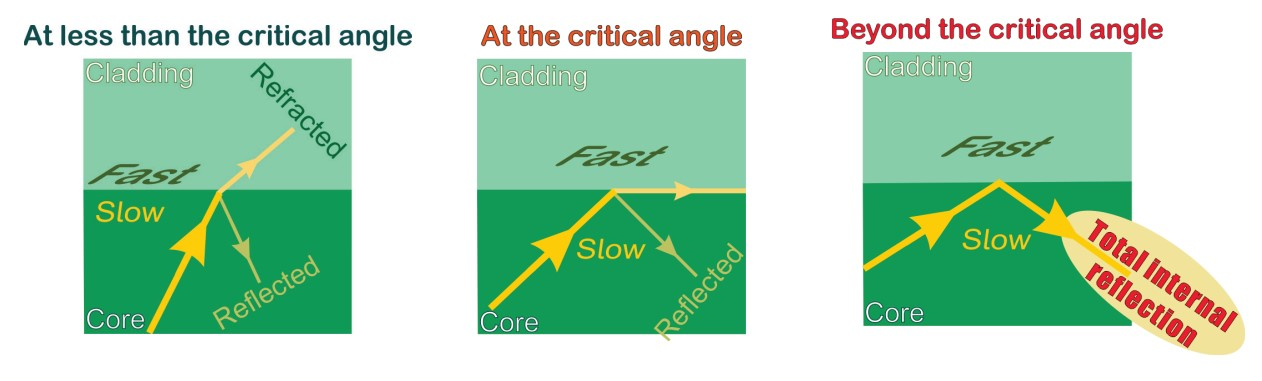
\includegraphics[width=\linewidth]{reflectionRefraction.jpg}

\section{Optical Fibres}
The core and cladding work together, to act like a pipe for light to bounce along. If the angle of the light is right, a beam of light will bounce along the core and will undergo total internal reflection whenever the light reaches the boundary between the core and cladding. \\
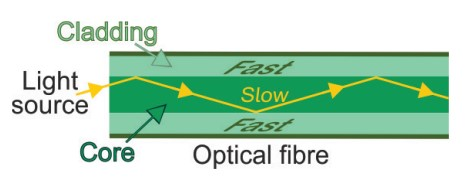
\includegraphics[width=\linewidth]{coreCladding.jpg}\\
The jacket adds mechanical strength to the fibre.
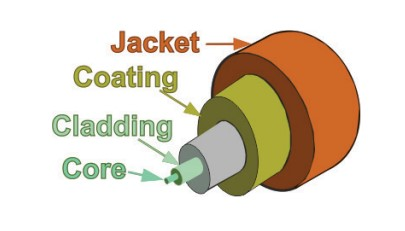
\includegraphics[width=\linewidth]{opticalFibre.jpg}
\subsection{Modes}
Optical fibre cables com in two modes. Mode refers to the way in which the light travels down the fibre.\\
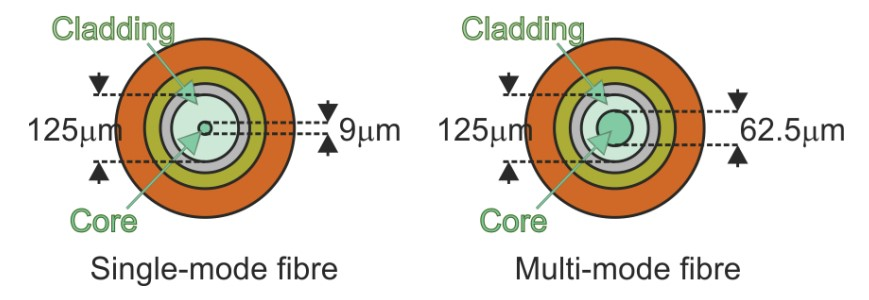
\includegraphics[width=\linewidth]{modes.jpg}
\subsubsection{Single-Mode Fibre}
In single-mode fibre, the light follows one path parallel to the length of the fibre. As only one signal is transmitted down at a time, the core is much thinner. Signals suffer less degradation therefore single-mode fibre is commonly used or long distance communication.
\subsubsection{Multi-Mode Fibre}
As this is fatter, it can allow multiple beams of light to move through it simultaneously, each following different paths (modes). There is greater signal degradation therefore this is only used for short distance communication.

\section{Optical Communication Systems}
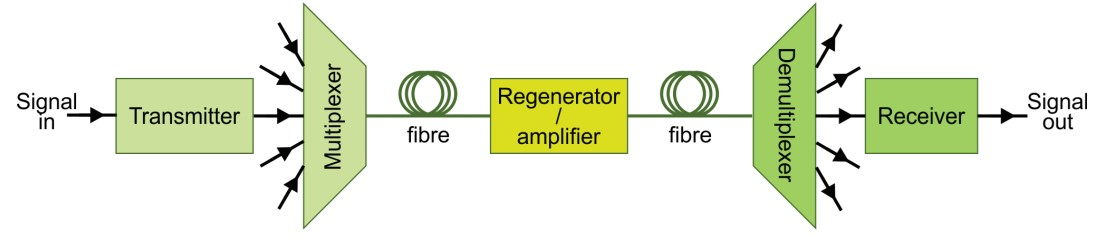
\includegraphics[width=\linewidth]{opticalCommSystems.jpg}\\
The signal is converted into a binary signal by the optical transmitter. The light pulses travel down an optical fibre and are received by a receiver which converts them back to electrical signals. Due to signal losses, longer cable runs require repeaters to regenerate the signals at regular intervals.
\subsection{Advantages And Disadvantages}
\subsubsection{Advantages}
Higher bandwidth than copper cable; immune to EM interference (therefore can operate in electrically noisy environments); highly secure as cannot be wire-tapped; signals can travel a long distance before they require regeneration; thinner, lighter and stronger than copper cables.
\subsubsection{Disadvantages}
They require specialist skills and technology to install and repair, which is expensive.
\subsection{Multiplexing}
To make the most efficient use of a communications link, signals are combined together musing multiplexing. At the end of the link, the signals are demultiplexed which separates the signals back to their original format. There are three different multiplexing techniques which can be used.
\subsubsection{Time Division Multiplexing}
Using this technique, each signal is given a time slot within a frame then all the signals are snt one after the other. This technique is also used in \textit{Pulse Code Modulation} systems.
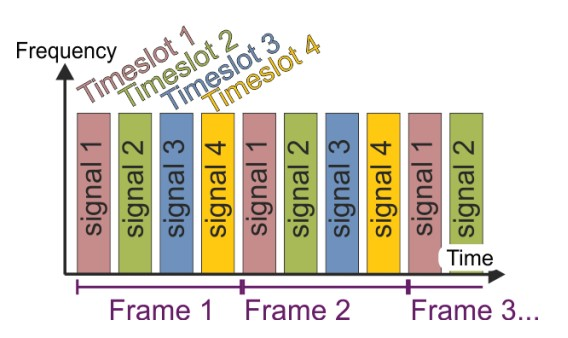
\includegraphics[width=\linewidth]{tdm.jpg}
\subsubsection{Frequency Division Multiplexing}
Using this technique, each signal is modulated onto a carrier signal. This allows multiple signals to transmit at the same time, using different carrier frequencies. This technique is also used in radio communication systems.
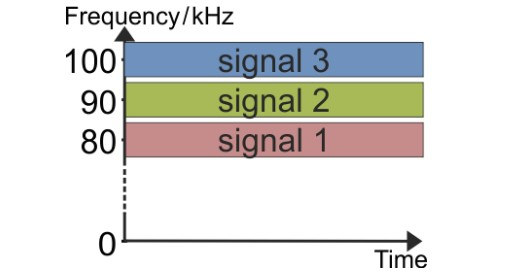
\includegraphics[width=\linewidth]{fdm.jpg}
\subsubsection{Wavelength Division Multiplexing}
This is very similar to FDM, except it uses wavelengths rather than frequencies. Using this technique, multiple different optical signals can be modulated onto different wavelength (different coloured) carriers. The individual signals then get separated at the other end of the communication link using optical filters. Wavelength ($\lambda$) is related to frequency ($f$) by $c = f \lambda$, where $c$ is the speed of light in the medium.
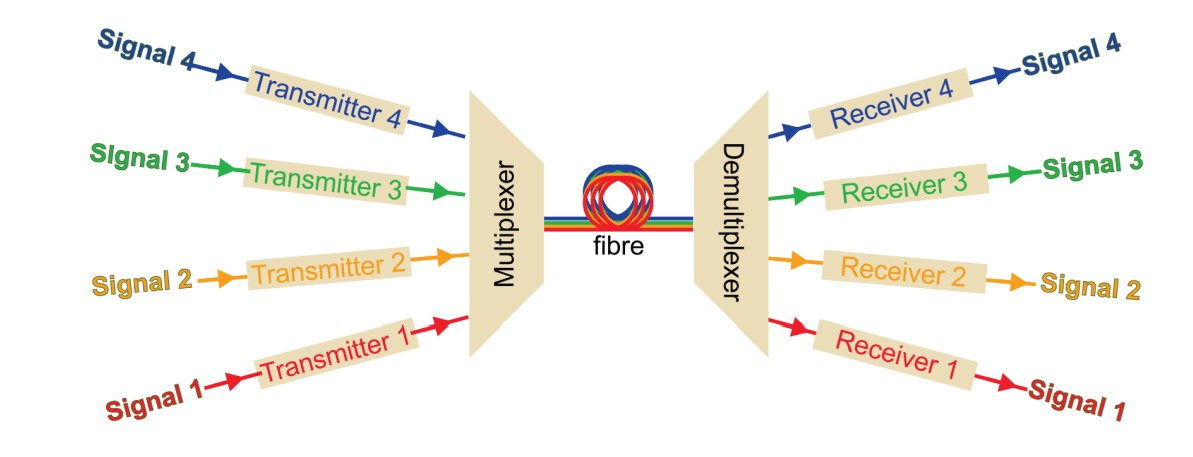
\includegraphics[width=\linewidth]{wdm.jpg}

\section{Losses In Optical Fibre}
There are two different ways which losses in the signal are introduced to optical communication links.
\subsection{Attenuation}
\textit{Attenuation is a reduction in signal level} and is expressed in decibels per kilometre ($dBkm^{-1}$).
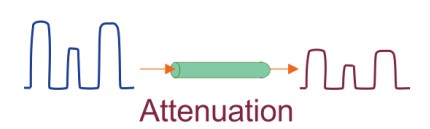
\includegraphics[width=\linewidth]{attenuationm.jpg}
\subsubsection{Causes}
Attenuation is caused by: absorption (where impurities in the core and cladding lead to some light being absorbed at particular wavelengths); scattering (where impurities in the glass can cause light rays to be scattered in different directions, decreasing the intensity of the beam in one direction); and bending loss (where as the cable is bent, the internal angles are changed therefore total internal reflection cannot happen meaning light gets refracted and signals are lost).
\subsection{Dispersion}
\textit{Dispersion is where the signal pulses are spread out over time} which limits the possible bit-rate of the signal as it becomes harder to distinguish between on and off pulses.
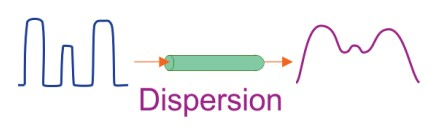
\includegraphics[width=\linewidth]{dispersion.jpg}
\subsubsection{Types Of Dispersion}
There are two different types of dispersion.
\paragraph{Modal Dispersion} 
When multi-mode fibre is used and multiple beams of light are being transmitted, each has its own path which is a different length to all the other ones. When the signals recombine, the original sharp pulse of light is spread into a less distinct signal.\\
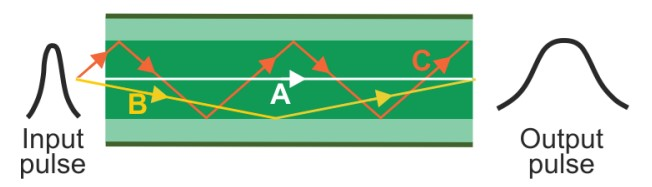
\includegraphics[width=\linewidth]{modalDisp.jpg}\\
One way to overcome this is to use singal mode fibre.
\paragraph{Chromatic Dispersion}
The speed of light in a medium depends on its wavelength (depends on its colour) therefore if a light source contains a range of wavelengths, each wavelength will take a different path and thus the pulse will be spread out when they recombine.\\
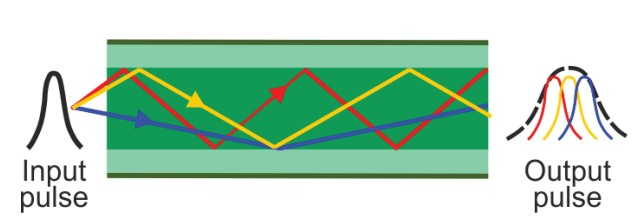
\includegraphics[width=\linewidth]{chromaticDisp.jpg}\\
One way to overcome this is to uses a laser light source as they contain a narrower range of wavelengths than a LED light source.
\subsection{Measuring Losses}
Power gain (or attenuation) can be expressed in Decibels (dB).\\
$\displaystyle G_{dB} = 10\log_{10}\left(\displaystyle \frac{P_{OUT}}{P_{IN}} \right)$\\
The ratio of actual signal to noise (signal-to-noise ratio) can be expressed in decibels.
\begin{align*}
    SNR_{dB} &= 10\log_{10} \left( \frac{P_S}{P_N} \right)\\
    SNR_{dB} &= 20\log_{10} \left( \frac{V_S}{V_N} \right)
\end{align*}

\section{Optical Technology}
\subsection{Light Sources}
Light sources for fibre-optic communications must be able to transmit light at an appropriate wavelength and be capable of being modulated fast enough to send data.
\subsubsection{LEDs}
LEDs contain a p-n junction that emits light when in forward bias. The colour emitted depends on the band-gap of the semiconductor. LEDs emit a wider range of frequencies than lasers therefore they are more susceptible to chromatic dispersion.
\subsubsection{Laser Diodes}
Light is generated at a p-n junction in the same way as in a LED. The light then bounces back and forth in a resonant cavity and is amplified, some of the light escapes as a monochromatic beam. Laser diodes are very high powered and require a heat sink.
\subsubsection{Comparison}
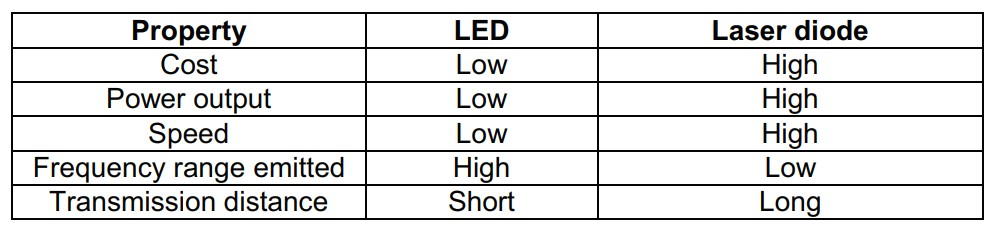
\includegraphics[width=\linewidth]{comparisonOfLaserLED.jpg}
LEDs are more robust therefore able to last for longer, they are also 20-30 times mor efficient than a laser diode. Laser diodes can be switched faster than LEDs so can transmit higher data rates. LEDs emit light over a broader area than lasers to less power is put into the fibre; limiting LEDs usage to multi-mode fibres and short distances.
\subsection{Optical Transmitters}
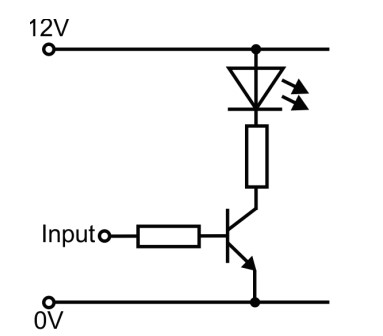
\includegraphics[width=\linewidth]{transmitterBJT.jpg}\\
The LED is switched on and off by the transistor, controlled by the input signal. Logic 1 causes the transistor to saturate, switching on the LED. The power consumed by the LED can be calculated using the voltage drop $V_F$ across the LED and the current calculated using the value of the current-limiting resistor. Alternatively, a MOSFET could be used.
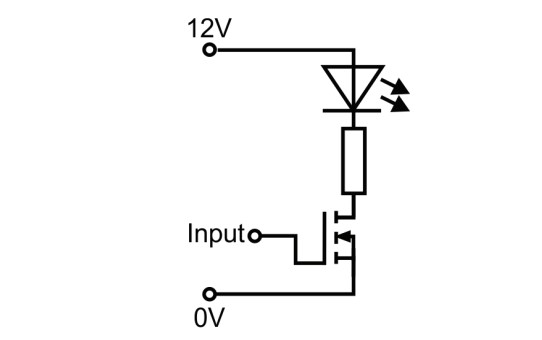
\includegraphics[width=\linewidth]{transmitterMOSFET.jpg}
\subsection{Detectors}
There are two different designs of detectors.
\subsubsection{Photodiode Detector}
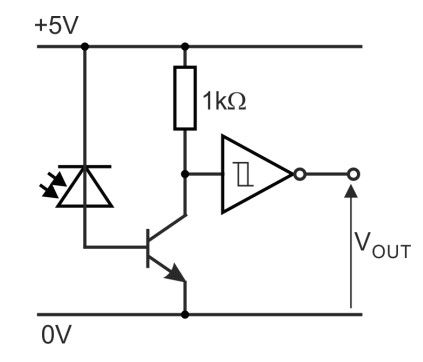
\includegraphics[width=\linewidth]{detectorPhotodiode.jpg}
The photodiode is in reverse bias so that when light hits it, a small current flows to the base of the transistor. This causes the transistor to switch on, causing the voltage at the collector to drop to zero. This is converted into an `on' pulse by the Schmitt inverter which cleans up the signal.
\subsubsection{Op-Amp Detector}
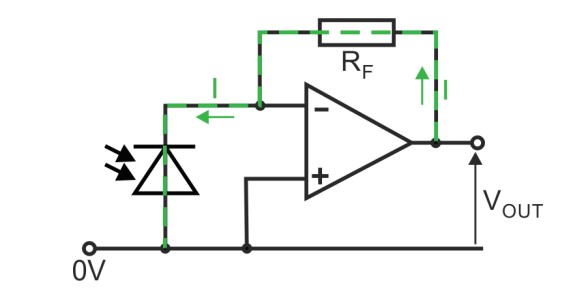
\includegraphics[width=\linewidth]{detectorOpAmp.jpg}
As op-amp inputs draw no current, when light falls on the photodiode, the current flows through $R_F$ from the output. Since the voltages at the two inputs of the op-amp must be equal, they must both be 0V therefore the voltage across $R_F$ is the same as $V_{OUT}$. This means that $V_{OUT} = I \times R_F$. This is a current-to-voltage converter (the current generated in the photodiode is converted into a voltage at the output).
\end{document}